\Chapter{Egy étterem, egy futár, több kiszállítás esete}

\Section{A probléma megfogalmazása}

Egy étterem, egy futár és több kiszállításnál az adott helyzet egészen visszavezethető a klasszikus utazó ügynök problémához.
A futár elindul az étteremből, érinteni kell az összes kiszállítási pontot, valamint vissza kell érkeznie az étterembe, mindezt úgy, hogy a lehető legkisebb utat tegye meg.
A probléma szemléltetése \aref{fig:model2}. ábrán látható.\cite{Diagrams.net}

\begin{figure}[h!]
\centering
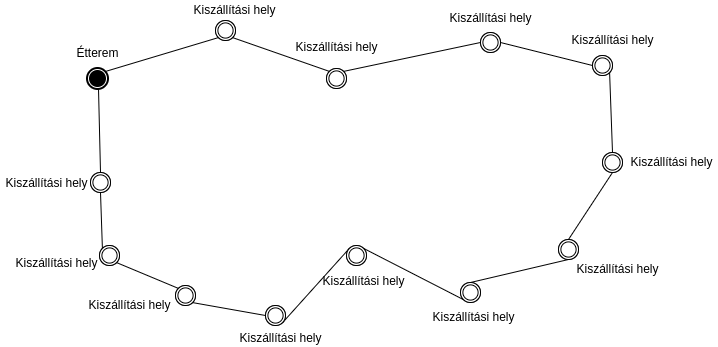
\includegraphics[scale=0.5]{images/Simpletsp.png}
\caption{Egy étterem, egy futár, több kiszállítás modellje}
\label{fig:model2}
\end{figure}

\Section{A probléma megoldása}

A probléma megoldásához egy nem determinisztikus módszer került implementálásra.
Ebben egy úgynevezett \textit{Gibbs-faktor} reprezentálja az új állapotba való áttérés valószí\-nű\-ségét.\cite{GibbsFactor}

A klasszikus utazó ügynök probléma matematikai megfogalmazása kiszállítási krité\-riumokra levetítve a következő.
Az egy ügynökös utazó ügynök probléma esetén jelölje $V$ a csúcsok (pontok) halmazát, $x_{i,j}$ azt, hogy az $i.$ pontból megy-e közvetlenül út a $j.$ pontba. Az $x_{i,j}$ értéke 1, ha útvonal köti össze a két pontot, különben 0: \cite{TSP}
\[
x_{i, j} \in \{0, 1\}, \quad i, j = 1, 2, \ldots, n, i \neq j.
\]

A $d_{i,j}$ jelöli az $i.$ és a $j.$ pont távolságát, $n$ pedig a pontok számát. A célfüggvény az alábbi:
\[
\displaystyle
\min \sum_{i=1}^n \sum_{j=1}^n d_{i,j} x_{i,j}.
\]

A célfüggvénnyel magát a megtett távolságot szeretnénk optimalizálni. A pontba csak egy él fut be, tehát
\[
\displaystyle
\sum_{i=1}^n x_{i,j} = 1, \quad j = 1, 2, \ldots, n, i \neq j.
\]

Valamint, minden pontból csakis egy él távozik, vagyis
\[
\displaystyle
\sum_{j=1}^n x_{i,j} = 1, \quad i = 1, 2, \ldots, n, i \neq j.
\]

A sorrendiség a következő feltétel alapján érvényesül
\[
u_i - u_j + n x_{i,j} \leq n - 1, \quad j = 2, 3, \ldots, n, i \neq j.
\]

Itt $u_{i}$ az $i.$ pont, $u_{j}$ a $j.$ pont látogatási indexe, ahol az $i.$ pontot hamarabb keresi fel az futár mint a $j.$ pontot.

\Section{A megoldás implementálása}

Összes lehetséges út száma
\(
\dfrac{(n-1)!}{2}.
\)
Ezek közül kell választanunk, ez ugyanis a Ha\-mil\-ton-körök száma az $n$ pontból álló teljes gráfban ($n > 2$ esetén).

A Python implementációhoz az alábbi import szükséges:\cite{Python} \cite{Spatial}
\begin{python}
from scipy.spatial import distance_matrix
\end{python}
A cél az, hogy listát készítsünk a pontokról, amelyek mindegyike két koordinátát tartalmaz $(x, y)$ formában, amelyek 0 és 100 közötti véletlen egész számokként kerülnek kiválasztásra. Jelen esetben 10 ilyen pont lesz.
\begin{python}
points = [random.sample(range(100), 2) for x in range(10)]
\end{python}
A pontok közötti távolságok kimutatását a program az alábbi módon oldja meg.
\begin{python}
data = Points
points = ['1', '2', '3', '4', '5', '6', '7', '8', '9', '10']
df = pd.DataFrame(data, columns=['xcord', 'ycord'], index=points)
pd.DataFrame(
	distance_matrix(
		df.values, 
		df.values
	), 
	index=df.index,
	columns=df.index
)
\end{python}

Ennek az eredménye \aref{fig:kimenet}. ábrán látható.

\begin{figure}[h!]
\centering
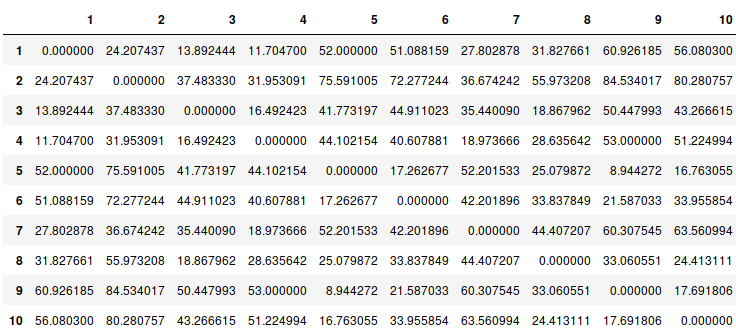
\includegraphics[width=\textwidth]{images/table.png}
\caption{Pontok közötti távolságmátrix}
\label{fig:kimenet}
\end{figure}

Inicializáljuk a \texttt{pointCount} értékét 10-re, ugyanis ennyi helyre kell a futárnak eljutnia.
\begin{python}
pointCount = 10
\end{python}
A \texttt{travel} egy adott számból álló lista (jelen esetben 10 számból áll), amely a pontok meglátogatására utal. Feltételezzük, hogy zárt hurokra van szükség, így az utolsó pont automatikusan csatlakozik az elsőhöz.
\begin{python}
travel = random.sample(range(pointCount), pointCount);}
\end{python}
Elindítunk egy ciklust az adott értékekkel
\begin{python}
for tlp in numpy.logspace(0, 5, num=100000)[::-1]:
\end{python}
Két pont véletlenszerű cseréjével új utat képzünk. Ezt úgy valósítom meg, hogy választok két számot az $i$-t és a $j$-t. Összeállítom a \texttt{newTravel}-t a régi travel másolásával az $i$ indexig, majd összefűzöm a $j$-edik \texttt{travel}-t és egészen folytatom addig, amíg a $j$ nem éri el az $i$-edik pontot, majd befejezem a \texttt{travel} többi részét.
\begin{python}
[i, j] = sorted(random.sample(range(pointCount), 2));
newTravel = travel[:i] + 
			travel[j:j + 1] + 
			travel[i + 1:j] + 
			travel[i:i + 1] + 
			travel[j + 1:]
\end{python}

Bizonyos valószínűséggel a \texttt{travel} megkapja a \texttt{newTravel} értékét, az előzöekben említett csere miatt ez már változott. Az elképzelés az, hogy minimalizálni szeretnénk a pontok közti távolságok költségének összegét. Ehhez a Gibb-s faktort használtam fel, aminek lényege, az új állapotba való átmenet valószínűsége. Csak az $i$-edik és $j$-edik pontok közötti távolságokat szükséges összegezni, mivel a többi távolság ugyanaz a \texttt{travel}-ben, mint a \texttt{newTravel}-ben. Ha a faktor értéke nagyobb, mint 1, akkor az új költség alacsonyabb, a \texttt{travel} megkapja a \texttt{newTravel} értékét.
Ez Python implementáció formájában a következőképpen néz ki.
\begin{python}
traveld = sum([
	math.sqrt(
		sum([(
			(
			  (points[travel[(k + 1) % pointCount]][d]) - 
			  (points[travel[k % pointCount]][d])
			) **  2
		) for d in [0, 1]])
	) for k in [j, j - 1, i, i - 1]
])
newTraveld = sum([
	math.sqrt(
		sum([(
			(
			  (points[newTravel[(k + 1) % pointCount]][d]) - 
			  (points[newTravel[k % pointCount]][d])) 
			** 2
		) for d in [0, 1]])
	) for k in [j, j - 1, i, i - 1]
])
if math.exp((traveld - newTraveld) / tlp) > random.random():
    travel = copy.copy(newTravel);
\end{python}
Az algoritmus végeztével már csak meg kell jeleníteni a kívánt pontokat, ez kirajzol egy gráfot, amely optimális utat ad. Ehhez a \texttt{matplotlib} függvénykönyvtárt használtam az alábbi módon.
\begin{python}
plt.plot(
	[points[
		travel[i % pointCount]][0] for i in range(pointCount + 1)
	], 
	[points[
		travel[i % pointCount]][1] for i in range(pointCount + 1)
	], 
	'xb-'
)
plt.show()
\end{python}

\Section{A megoldás tesztelése}

A \texttt{pointCount} állításával adhatjuk meg, hogy hány helyre is kell mennie a futárnak. Ennek módosításával több lefuttatott teszt után is megfigyelhető, hogy az összehasonlítások száma 65 ezer és 75 ezer között mozog. Egytől egyig az optimális utat adták. Mivel véletlenszerű számok összehasonlításán alapszik az algoritmus ezáltal az összehasonlítások száma igen magas, viszont stagnál bizonyos értékek között.

\Aref{fig:tsp5location}., \ref{fig:tsp10location}., \ref{fig:tsp15location}., \ref{fig:tsp20location}., \ref{fig:tsp25location}., \ref{fig:tsp30location}., \ref{fig:tsp35location}. és \ref{fig:tsp40location}. ábrákon különböző számú pont esetén meghatározott optimális utakat láthatunk.

\begin{figure}[h!]
\centering
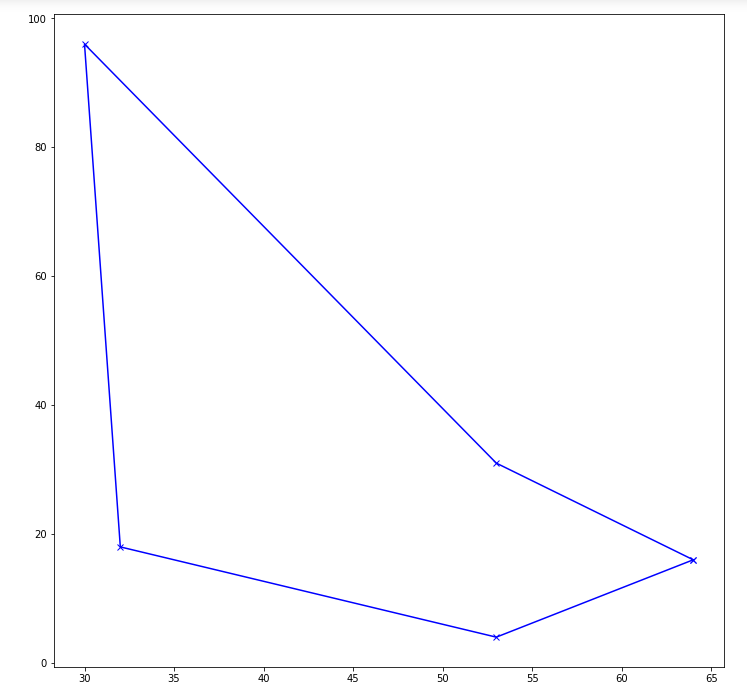
\includegraphics[scale=0.4]{images/5.png}
\caption{5 kiszállítási hely esetén az összehasonlítások száma: 74 434}
\label{fig:tsp5location}
\end{figure}

\begin{figure}[h!]
\centering
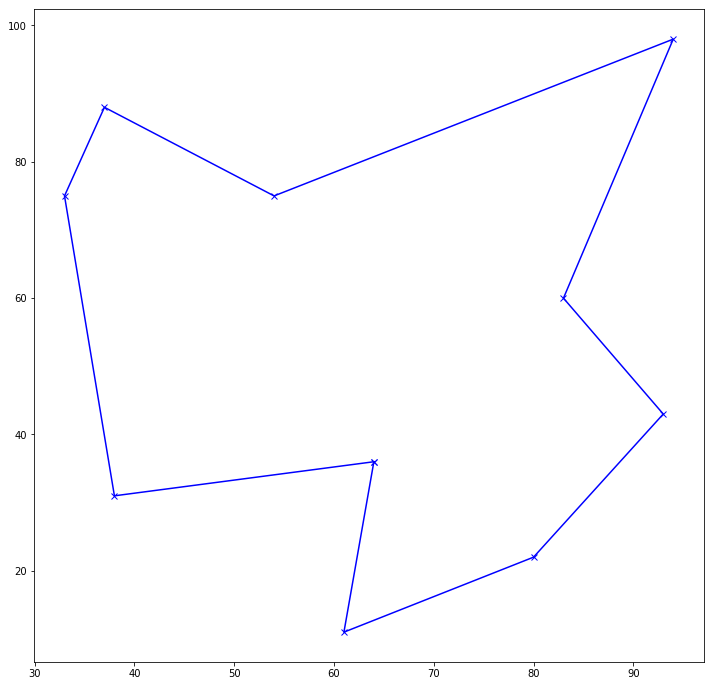
\includegraphics[scale=0.4]{images/10.png}
\caption{10 kiszállítási hely esetén az összehasonlítások száma: 68 594}
\label{fig:tsp10location}
\end{figure}

\begin{figure}[h!]
\centering
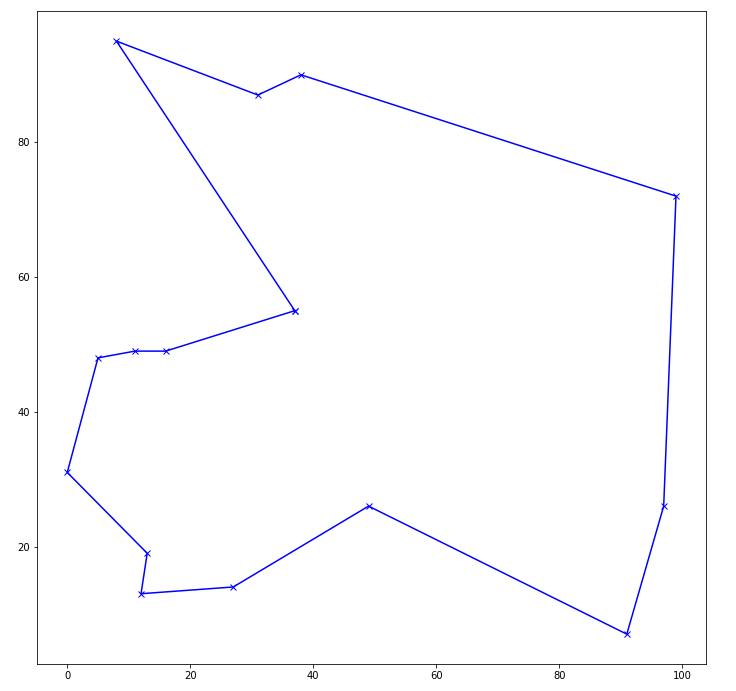
\includegraphics[scale=0.4]{images/15.png}
\caption{15 kiszállítási hely esetén az összehasonlítások száma: 66 672}
\label{fig:tsp15location}
\end{figure}

\begin{figure}[h!]
\centering
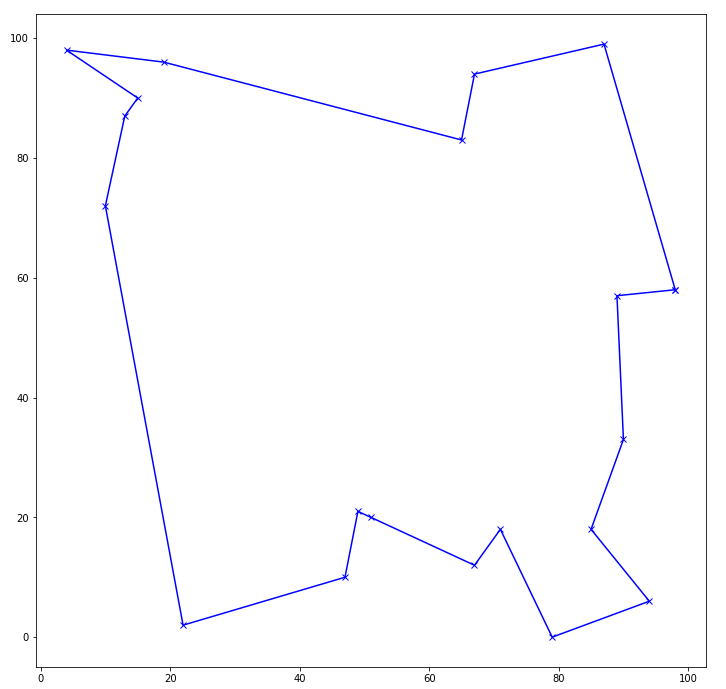
\includegraphics[scale=0.4]{images/20.png}
\caption{20 kiszállítási hely esetén az összehasonlítások száma: 65 265}
\label{fig:tsp20location}
\end{figure}

\begin{figure}[h!]
\centering
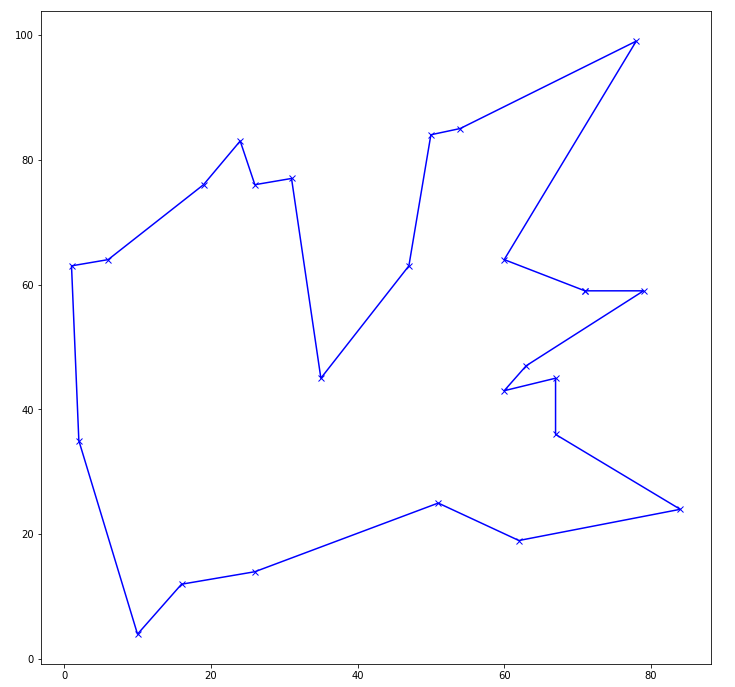
\includegraphics[scale=0.4]{images/25.png}
\caption{25 kiszállítási hely esetén az összehasonlítások száma: 67 865}
\label{fig:tsp25location}
\end{figure}

\begin{figure}[h!]
\centering
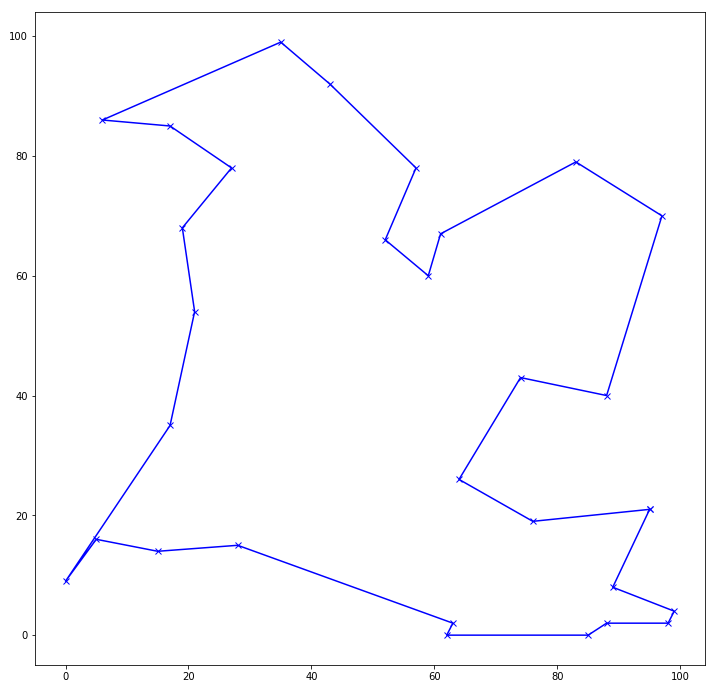
\includegraphics[scale=0.4]{images/30.png}
\caption{30 kiszállítási hely esetén az összehasonlítások száma: 65 324}
\label{fig:tsp30location}
\end{figure}

\begin{figure}[h!]
\centering
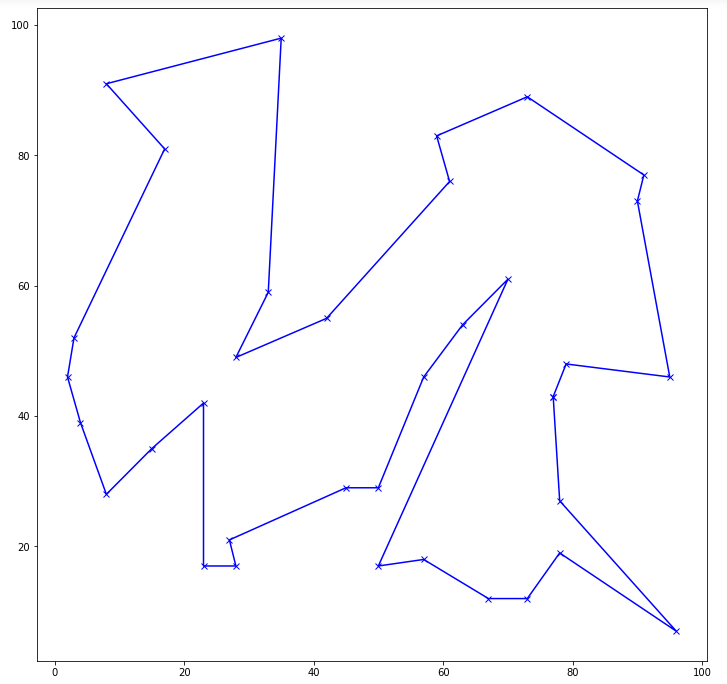
\includegraphics[scale=0.4]{images/35.png}
\caption{35 kiszállítási hely esetén az összehasonlítások száma: 67 230}
\label{fig:tsp35location}
\end{figure}

\begin{figure}[h!]
\centering
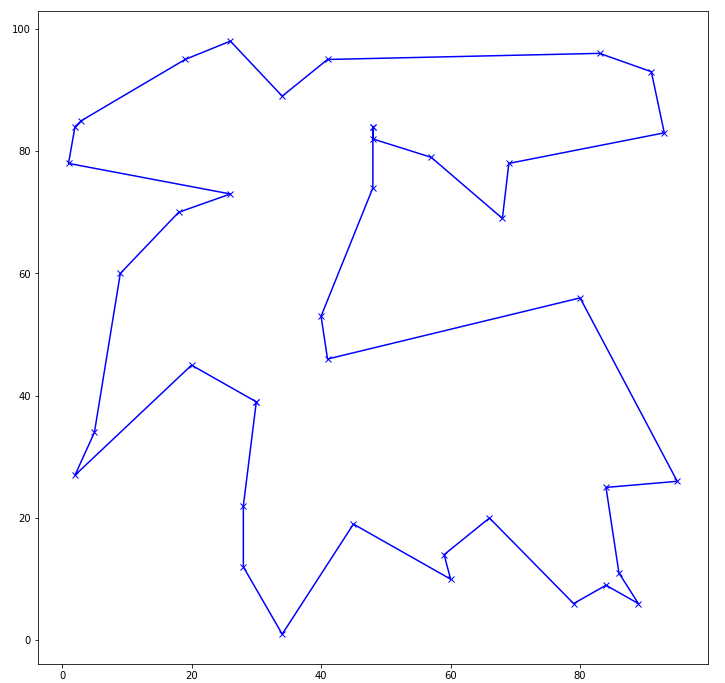
\includegraphics[scale=0.4]{images/40.png}
\caption{40 kiszállítási hely esetén az összehasonlítások száma: 66 008}
\label{fig:tsp40location}
\end{figure}

